\documentclass[english,serif,mathserif,usenames,dvipsnames]{beamer}
\usetheme[formal]{s3it}

% \usepackage[T1]{fontenc}
% \usepackage[utf8]{inputenc}
% \usepackage{babel}

%% This is optional: it adds a few commands and environment we
%% regularly use in our slide sets
\usepackage{s3it}
\usepackage{tikz}
\usepackage{caption}
% \usepackage{minipage}

\setbeamertemplate{itemize
  item}{\color{uzh@blue}\scriptsize\raise1.25pt\hbox{$\bullet$}}

\begin{document}

%% Optional Argument in [Brackets]: Short Title for Footline
\title[IaaS (OpenStack) overview]{IaaS Cloud (OpenStack) overview}

\author{%
  {\bfseries Antonio Messina \texttt{<antonio.messina@s3it.uzh.ch>}}  
}

\institute[UZH]{%
  S$^3$IT - Services and Support for Science IT,
  University of Zurich
}
\date{2~September~2014}

%% Makes the title slide
\maketitle

\begin{frame}
  {What is OpenStack}

  \begin{quote}
    OpenStack is a cloud operating system that controls large pools of
    compute, storage, and networking resources throughout a
    datacenter, all managed through a dashboard that gives
    administrators control while empowering their users to provision
    resources through a web interface.

    \hfill{\em \url{www.openstack.org}}
  \end{quote}
\end{frame}
% \begin{frame}[fragile]
%   {Cattle vs. pets}

%   \scriptsize
%   \begin{columns}
%     \column{0.5\linewidth}
%     
\includegraphics[width=\linewidth]{kitten}
%     \column{0.5\linewidth}
%       \begin{itemize}
%       \item pets are given names like \texttt{kenny.example.org}
%       \item you care about them
%       \item they are unique, you check on them every day
%       \item when they get ill, you nurse them back to health
%       \end{itemize}

%   \end{columns}
%   \+\+\+
%   \begin{columns}
%     \column{0.5\linewidth}
%     \visible<2->{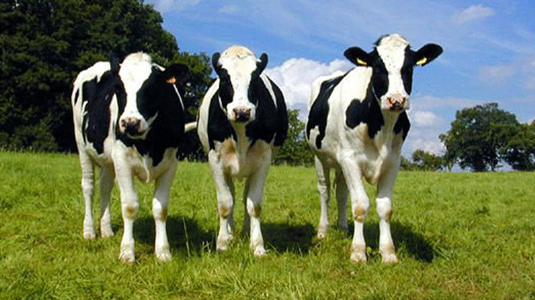
\includegraphics[width=\linewidth]{cattle}}

%     \column{0.5\linewidth}
%     \visible<2->{\begin{itemize}
%     \item cattle are given names like \texttt{vm-001.example.org}
%     \item they are all the same
%     \item when they get ill, you shoot them and get another one
%     \end{itemize}}
%   \end{columns}
%   % \includegraphics[width=\linewidth]{servers_pets_or_cattle.jpg}

%   % \tiny Rif: \url{http://www.slideshare.net/gmccance/cern-data-centre-evolution}
% \end{frame}

\begin{frame}
  {OpenStack vs. rest of the (virtualization) world}
  What's different from KVM/VMWare/Virtualbox?

  \begin{itemize}
    \pause
  \item specs of the VMs are choosen form a list of predefined
    \textbf{flavors} that define:
    \begin{itemize}
    \item Nr. of CPUs
    \item amount of RAM
    \item size disk
    \end{itemize}

    \pause
  \item complex network setup are possible

    \pause
  \item OS already installed (but adapted automatically to the current
    instance)

    \pause
  \item multiple options for storage (volumes and object storage)

    \pause
  \item VMs are spawned on possibly thousends of nodes

  \end{itemize}

\pause\scriptsize
    yes, it's a \textit{clone} of Amazon
\end{frame}

\begin{frame}
  {Above all}

  creation is done via Web GUI, CLI or \textbf{network APIs}

  $\Rightarrow$ it can be \textit{scripted}

  \+
  \pause
  You just have to setup the cloud.

  \+
  Actual provisioning of the VMs can be delegated \textbf{to
    the user}


\end{frame}

\begin{frame}
  {OpenStack Architecture}
  \begin{itemize}
  \item written in Python (plus auxiliary shell scripts)
  \item built around \textbf{independent components}
  \item \textbf{highly distributed} architecture
    \begin{itemize}
    \item designed for very big installations
    \end{itemize}
  \item \textbf{intrinsic HA} of \textit{most} OpenStack services (MySQL and
    RabbitMQ have to be properly configured)
  \item \textbf{*SQL} database used to store persistent data
  \item \textbf{RabbitMQ} used for RPC and notification
  \item \textbf{RESTful APIs} for all the services
  \end{itemize}
\end{frame}


\begin{frame}
  {OpenStack logical view}
  
  \begin{tikzpicture}
    \node (0,0){
      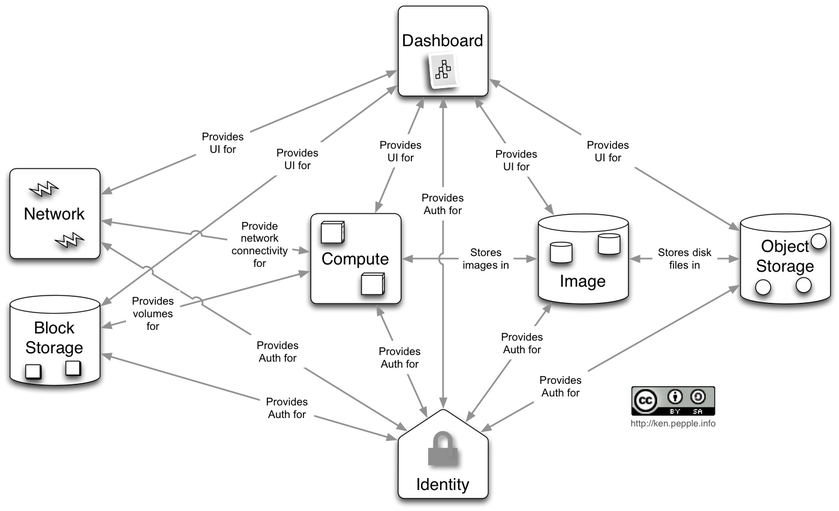
\includegraphics[width=\linewidth]{openstack-conceptual-arch.png}};
    % identity
    \visible<2>{\draw[red, fill=red, opacity=0.3] (0.25,-2.5) circle (0.9);}
    % compute
    \visible<3>{\draw[red, fill=red, opacity=0.3] (-0.8,-0.05) circle (0.9);}
    % neutron
    \visible<4>{\draw[red, fill=red, opacity=0.3] (-4.5,0.5) circle (0.9);}
    % image
    \visible<5>{\draw[red, fill=red, opacity=0.3] (2,-0.05) circle (0.9);}
    % block
    \visible<6>{\draw[red, fill=red, opacity=0.3] (-4.5,-1.1) circle (0.9);}
    % object
    \visible<7>{\draw[red, fill=red, opacity=0.3] (4.48,-0.05) circle (0.9);}
    % dashboard
    \visible<8>{\draw[red, fill=red, opacity=0.3] (0.3,2.5) circle (0.9);}
  \end{tikzpicture}

  \alt<1>{\vspace{1.4em}}{~}
  \alt<2>{\textbf{Keystone} provides the authentication service}{}
  \alt<3>{\textbf{Nova} provides computational services}{}
  \alt<4>{\textbf{Neutron} provides network services}{}
  \alt<5>{\textbf{Glance} provides image store}{}
  \alt<6>{\textbf{Cinder} provides block persistent store}{}
  \alt<7>{\textbf{Swift} provides object persistent store}{}
  \alt<8>{\textbf{Horizon} provides web user interface}{}
\end{frame}

\begin{frame}
  {keystone - authentication service}

  \begin{itemize}
  \item It's the \textbf{entry point} for OpenStack API.
  \item Stores authentication information (\textit{users},
    \textit{passwords}, \textit{tokens}, \textit{projects},
    \textit{roles})
  \item Holds a catalog of available services and their endpoints.
  \item Can use different backends (SQL database, LDAP)
  \end{itemize}
\end{frame}

\begin{frame}
  {nova - compute service}
  \begin{columns}
    \column{2cm}
    
\includegraphics[width=2cm]{openstack-compute-icon.png}
    \column{8cm}
    Service responsible of managing virtual instances.
  \end{columns}
  \begin{description}
  \item[nova-api] Web API frontend, accepts requests, validates them
    and contact other services if needed.
  \item[nova-scheduler] decides where to start an instance
  \item[nova-compute] running on each compute node, interacts with the
    hypervisor and actually starts the vm.
  \end{description}
\end{frame}

\begin{frame}
  {glance - image service}
  \begin{columns}
    \column{2cm}
    
\includegraphics[width=2cm]{glance-icon.png}
    \column{8cm}
    Service responsible of storing image informations and, optionally,
    image files.
  \end{columns}

  \+
  \begin{itemize}
  \item Holds information about available images.
  \item Optionally allow to download and upload images.
  \item Images can be stored on \textbf{different backends} (RDB, S3,
    Swift, filesystem)
  \end{itemize}
\end{frame}


\begin{frame}
  {neutron - network service}

  \begin{columns}
    \column{2cm}
    
\includegraphics[width=2cm]{openstack-networking-icon.png}
    \column{8cm}
    Service responsible of creating and managing networks. It is
    supposed to replace.
  \end{columns}

  \+\+
  Still not widely used, but very feature rich.


  \begin{itemize}
  \item L2 and L3 networks.
  \item Allow creation of multiple networks and subnets.
  \item Plugin architecture.
  \item Supports advanced network services (Load Balancer, Firwall,
    DNS as a service)
  \item Integrates with network devices (Cisco, Brocade\ldots)
  \end{itemize}
\end{frame}


\begin{frame}
  {cinder - block storage}
  \begin{columns}
    \column{2cm}
    
\includegraphics[width=2cm]{block_storage.png}
    \column{9cm}
    \begin{itemize}
    \item Creates and export volumes via iSCSI to the compute node.
    \item Volumes are mounted \textbf{transparently} from the virtual
      machines.
    \item Supports \textbf{multiple storage backends} (NFS, LVM, Ceph,
      GlusterFS but also SAN/NAS devices from IBM, NetApp etc\ldots )
    \end{itemize}
  \end{columns}

  \+
  composed of \textbf{multiple services}:
  \begin{description}
  \item[cinder-api] Web API frontend.
  \item[cinder-volume] Manages block storage devices. You can have
    many of these.
  \item[cinder-scheduler] Decides which cinder-volume has to provide
    the volume for an instance.
  \end{description}
\end{frame}


\begin{frame}
  {swift - object storage}
  \begin{columns}
    \column{2cm}
    
\includegraphics[width=2cm]{openstack-object-storage-icon.png}
    \column{8cm}
    Object storage distributed service.
  \end{columns}
  
  \+\+
  \begin{itemize}
  \item Redundant, scalable object storage on commodity hardware.
  \item Not a POSIX filesystem.
  \item Scales horizontally simply by adding new servers.
  \end{itemize}

  \+ It's not the only choice: \textbf{Ceph}, \textbf{GlusterFS} and
  others can be used instead.

\end{frame}

\begin{frame}
  {Life of a virtual machine}

  \begin{enumerate}

  \item \alt<2>{\HL{Authentication is performed}}{Authentication is
      performed} either by the web interface \textbf{horizon} or
    \textbf{nova} command line tool: \alt<2>{
    \begin{enumerate}
      \item keystone is contacted and authentication is performed
      \item a \textbf{token} is saved in the database and returned to
        the client to be used with later
        interactions with OpenStack services for this request.
      \end{enumerate}
      }{}
    \item \alt<3>{\HL{\textbf{nova-api} is
          contacted}}{\textbf{nova-api} is contacted} and a new request
        is created:

    \alt<3>{
      \begin{enumerate}
      \item checks via \textbf{keystone} the validity of the token
      \item checks the authorization of the user
      \item validates parameters and create a new request in the
        database
      \item calls the scheduler via queue
      \end{enumerate}
      }{}

  \item \alt<4>{\HL{\textbf{nova-scheduler} find an appropriate host}}{\textbf{nova-scheduler} find an appropriate host}

    \alt<4>{
      \begin{enumerate}
      \item reads the request
      \item find an appropriate host via filtering and weighting
      \item calls the chosen \textbf{nova-compute} host via queue
      \end{enumerate}
    }{}
 
\item \alt<5>{
    \HL{\textbf{nova-compute}} reads the request and \HL{start an
      instance}:}
  {\textbf{nova-compute} reads the request and start an instance:}

  \alt<5>{
    \begin{enumerate}
    \item generates a proper configuration for the hypervisor
    \item get image URI via image id
    \item download the image
    \item request to allocate network via queue
    \end{enumerate}
    }{}

\item \alt<6>{\HL{\textbf{nova-compute} contacts \textbf{cinder}} to
      provision the volume} (if requested)
  {\textbf{nova-compute} contacts \textbf{cinder} to provision the volume}

  \alt<6>{
    \begin{enumerate}
    \item gets connection parameters from cinder
    \item uses iscsi to make the volume available on the local machine
    \item asks the hypervisor to provision the local volume as virtual
      volume of the specified virtual machine
    \end{enumerate}
  }{}

\item \alt<7>{\HL{\textbf{neutron} configure the network}}
    {\textbf{neutron} configure the network}
  \alt<7>{
    \begin{enumerate}
    \item allocates a valid private ip
    \item if requested, it allocates a floating ip
    \item configures the host as needed (dnsmasq, iptables,
      Open VSwitch\ldots)
    \item updates the request status
    \end{enumerate}
  }{}

\item \alt<8>{\HL{\textbf{nova-compute} starts the virtual machine}}
  {\textbf{nova-compute} starts the virtual machine}

\item \alt<9>{\HL{\textbf{horizon/nova} poll \textbf{nova-api}}}
  {\textbf{horizon/nova} poll \textbf{nova-api}} 
  until the VM is ready.
 \end{enumerate}

\end{frame}


\begin{frame}
  {Notes on installation}

  \begin{itemize}
  \item Please, please, please, use a \textbf{deployment and
      configuration manager}. There are many:
    \href{http://puppetlabs.com/}{Puppet},
    \href{http://www.getchef.com/}{Chef},
    \href{http://cfengine.com/}{CFEngine},
    \href{http://www.ansible.com/home}{Ansible},
    \href{http://www.saltstack.com/}{SaltStack}\ldots~ Just pick the
    one you like most.
  \item Do not underestimate the \textbf{complexity} of the system.
  \item Plan in advance, and \textbf{plan for failures}.
  \item RTFM: the OpenStack website is now plenty of
    documentation\footnote{\scriptsize it wasn't like this 2 years ago\ldots}
    \begin{itemize}
    \item
      \href{http://docs.openstack.org/icehouse/install-guide/install/apt/content/index.html}{Install
        Guide (for Ubuntu 12.04/14.04)}
    \item
      \href{http://docs.openstack.org/arch-design/content/index.html}{Architecture
        Design Guide}
    \item
      \href{http://docs.openstack.org/admin-guide-cloud/content/}{Cloud
        Administrator Guide}
    \item
      \href{http://docs.openstack.org/training-guides/content/}{Training guide}
    \item \href{http://docs.openstack.org/openstack-ops/content/}{Operations Guide}
    \item
      \href{http://docs.openstack.org/high-availability-guide/content/index.html}{High
        Availability Guide}
    \item
      \href{http://docs.openstack.org/security-guide/content/}{Security Guide}
    \end{itemize}
  \end{itemize}

\end{frame}


\begin{frame}
  {OpenStack software overview}
  \begin{figure}[ht]
    \centering
    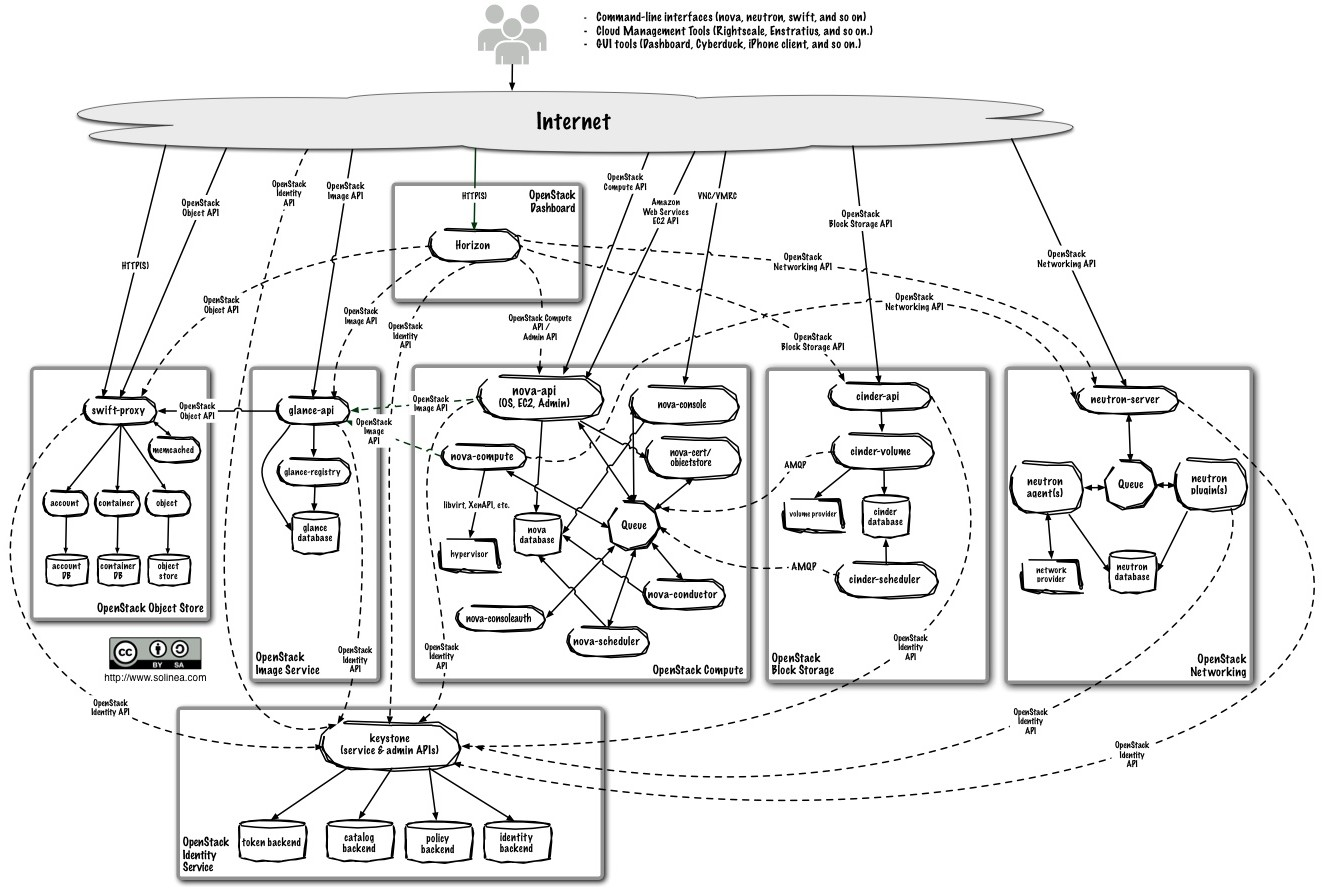
\includegraphics[width=\linewidth]{openstack-arch-havana-logical-v1.jpg}
    
  \caption*{\href{http://docs.openstack.org/training-guides/content/figures/5/a/figures/openstack-arch-havana-logical-v1.jpg}{OpenStack software overview}}
\end{figure}
\end{frame}

\begin{frame}
  {Other OpenStack services}
  Projects \textbf{integrated} in Icehouse:
  \begin{itemize}
  \item \href{https://wiki.openstack.org/wiki/Ceilometer}{Ceilometer}
    (Metering)
  \item \href{https://wiki.openstack.org/wiki/Heat}{Heat}
    (Orchestration)
  \item \href{https://wiki.openstack.org/wiki/Trove}{Trove} (Database
    as a service)
  \item \href{https://wiki.openstack.org/wiki/Sahara}{Sahara} (Data
    Processing - Hadoop)
  \end{itemize}

\+
  Projects in \textbf{incubation}:
  \begin{itemize}
  \item \href{https://wiki.openstack.org/wiki/Ironic}{Ironic} (Bare
    metal provisioning)
  \item \href{https://wiki.openstack.org/wiki/Zaqar}{Zaqar (aka
      \textit{Marconi})} (Messaging service)
  \item \href{https://wiki.openstack.org/wiki/Barbican}{Barbican}
    (Secure storage of secrets)
  \item \href{https://wiki.openstack.org/wiki/Designate}{Designate} (DNSaaS)
  \item \href{https://wiki.openstack.org/wiki/TripleO}{TripleO} (OpenStack-on-OpenStack)
  \end{itemize}
\end{frame}
\end{document}

%%% Local Variables:
%%% mode: latex
%%% TeX-master: t
%%% End:
